\documentclass[preprint]{sig-alternate-10pt}

\usepackage{cite}
\usepackage{graphicx}
\usepackage{algorithm,algpseudocode}
\usepackage{algorithmicx}


\usepackage{amssymb}
\usepackage{mathrsfs}
\usepackage{amsmath}


\usepackage[sans]{dsfont}
\usepackage{stmaryrd}
\usepackage{pifont}
\usepackage{wasysym}

\usepackage{array}
\usepackage{url}
\usepackage[usenames]{color}
\usepackage[tight,footnotesize]{subfigure}


\usepackage{xcolor}
\usepackage{listings}
\usepackage {tikz}
\usetikzlibrary {positioning}
\definecolor {processblue}{cmyk}{0.96,0,0,0}
\usepackage{setspace}


\renewcommand{\algorithmicrequire}{\textbf{Input:}}
\renewcommand{\algorithmicensure}{\textbf{Output:}}

\newtheorem{example}{Example}
\newtheorem{definition}{Definition}
\newtheorem{conjecture}{Conjecture}
\newtheorem{lemma}{Lemma}
\newtheorem{theorem}{Theorem}
\newtheorem{corollary}[theorem]{Corollary}
\newtheorem{proposition}[theorem]{Proposition}
\def\endexam{\hspace*{\fill}~$\diamond$\par\endtrivlist\unskip}

\setlength{\pdfpagewidth}{8.5in}
\setlength{\pdfpageheight}{11in}



\begin{document}


\title{Improving Building Energy Efficiency by Kinect-based Occupancy
  Tracking and Mobility Detection System}

\numberofauthors{1}
\author{\alignauthor  \ \\
\affaddr{some authors} \\
%\email{%\{\}@masdar.ac.ae}
}


\makeatletter
\let\@copyrightspace\relax
\makeatother

\pagestyle{plain}
\thispagestyle{plain}

\maketitle


\begin{abstract}
In an average open office building, air conditioning, ventilation and
lighting account for 30 to 40 percent of energy consumption. Nowadays,
most modern conditioning systems in buildings still operate based on
occupancy rather than actual usage. Such operation mode creates
needless conditioning and energy waste. Therefore, in order to achieve
an optimal conditioning state based on  traffic in zones of interest,
we need to know the rate and time of occupancy and intelligently tune
the system according to the  number of actual occupants.  In our
study, we use a people counting software based on a network of
Microsoft Kinect for Windows sensors in order to acquire temporal
occupancy information. The occupancy counter software provides
real-time occupancy data through detection and tracking of people in
the building.  An HVAC management and control system needs to adjust
this data in real-time and measure the local level of comfort.  In
this research, we propose an approach for energy saving which
integrates a real-time occupancy data into building management
systems. This approach leads us to the creation of an occupancy
monitoring and control system which takes into account three elements:
subject mobility, room status (e.g. empty, occupied, crowded) and
actual number of people.  In addition, in order to model the occupancy
data collected, we use the Markov chain principle where a state is a
combination of the statuses of existing zones in the building. Such
state represents the level of energy consumption in real time and a
useful input data for the HVAC system controller.  Here, we
demonstrate that our model, based on data collected by an ensemble of
Kinect sensors, can be integrated with an HVAC control strategy to
achieve substantial energy savings. Through the prediction of future
occupancy level of particular zones of a building, our intelligent
system is able to adjust conditioning parameters gradually to reflect
the predicted changes in time.  
\end{abstract}


\noindent
{\bf Categories and Subjects:} {[Computer systems organization]}: {\em Embedded and cyber-physical systems}: {\em Sensors and actuators}

\noindent
{\bf General Terms: }Algorithms, Design, Management


\noindent
{\bf Keywords: }Wireless Sensor Networks.
\\

\section{Introduction} \label{sec:intro}

As automotive information systems read and process more data from vehicles and their environments, so too have increased the consumer expectations of useful information from these systems, often in real time. Among these is the estimation of future fuel consumption, which is typically combined with known information about fuel tank capacity and provided to drivers in the form of a Distance-to-Empty (DTE) readout. Accurate prediction of fuel consumption, and thereby DTE, is vital in allowing drivers to know not only when they need to refuel, but also the fuel consumption along different possible routes.

\cite{rodgersetal2013} describes the use of a linear regression technique to predict DTE for electric vehicles. The technique can be adapted for use with internal combustion vehicles to predict their fuel consumption along routes they have driven, based on modeled driving behavior and driving conditions. However, all drivers will not have driven along all possible routes. One driver \(A\) may be interested in finding out how much fuel she is likely to consume along a route \(X\) she has never driven previously. However, if other drivers \(B\) and \(C\) have driven route \(X\), along with other routes \(Y\) and \(Z\) also driven by \(A\), we can use the aforementioned technique to model the differences among the routes, and the differences among the drivers' fuel consumption patterns on the same routes. Combining these models allows us to predict the fuel consumption of driver \(A\) over \(X\).

\input{background}
\section{Design and Implementation}
\label{sec:design}


\subsection{Kinect-based Occupancy Counter }
Our  Occupancy Counter software is written using Microsoft Visual $C\sharp$ 2010,  project WPF application programmed using $C\sharp$ and XML languages.  OS used is Windows 7 with Kinect Studio v. 1. 7. 0 and Developer Toolkit Browser v. 1. 7. 0 installed.  Both type of Kinect is used and tested to be running on our software,  Xbox Kinect and Kinect for windows.  The software,  should be run in windows 7 or above,  with pre---installation of Kinect sensor drivers \emph{(shortly by installing Kinect SDK)}.

 \begin{figure}[!ht]
  \begin{center}
	  	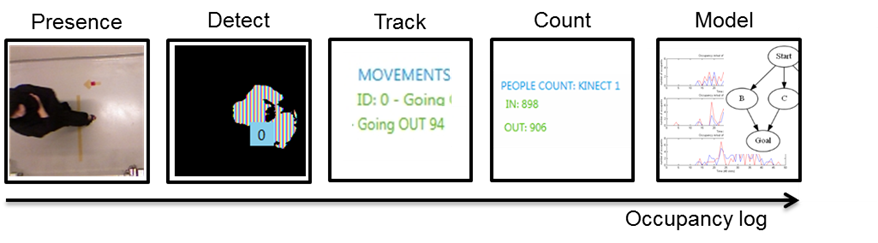
\includegraphics[width=1\columnwidth]{./images/112200.png}
  \end{center}
  \caption{Human detection,  tracking, counting and analysis}
\end{figure}

\begin{enumerate}
  \item \textbf{Kinect initialization start:} This function will look up for any connected Kinect devices to your computer.  If no device is connected: a box message will appear to inform you about this fact.  The software display both RGB and Depth image,  Figure \ref{fig:guioverview} show the GUI of our software.

     \begin{figure}[!ht]
  \begin{center}
	  	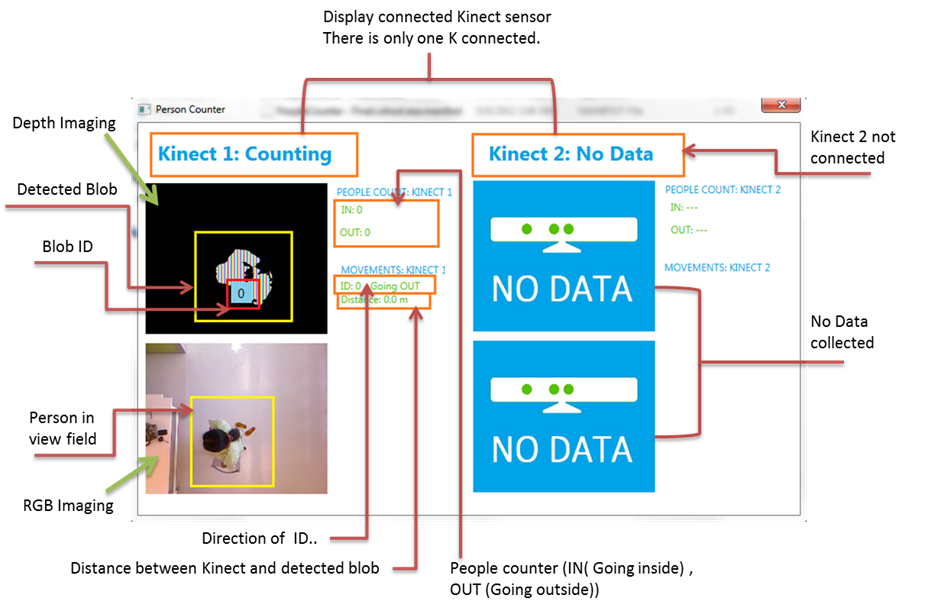
\includegraphics[width=1.1\columnwidth]{./images/swm.png}
  \end{center}
  \caption{Overview of the GUI of our Kinect-based Occupancy Counter x.}
  \label{fig:guioverview}
\end{figure}
\item \textbf{Capture frame events}: As part of the initialization,  it makes sure that both RGB and Depth imaging are captured.
ColorImageFrameReadyEventArgs:	The event arguments provided in a KinectSensor. ColorFrameReady event when a frame of color data is ready.
\item \textbf{Depth camera feed generator:} Contains a per-frame buffer for depth data streamed out of a sensor.  Also provides access to the dimensions and format of the data in addition to mapping between skeleton and color coordinate spaces.  Once our Depth imaging is ready, we can start tracking blobs and draw markers.
\item \textbf{Generate Markers :} This draws a rectangle blue box  with unique ID of people that is used is temporarily  for the detection of multiple subjects passing in the field view.

\end{enumerate}


\begin{figure} [!ht]
  \begin{center}
	  	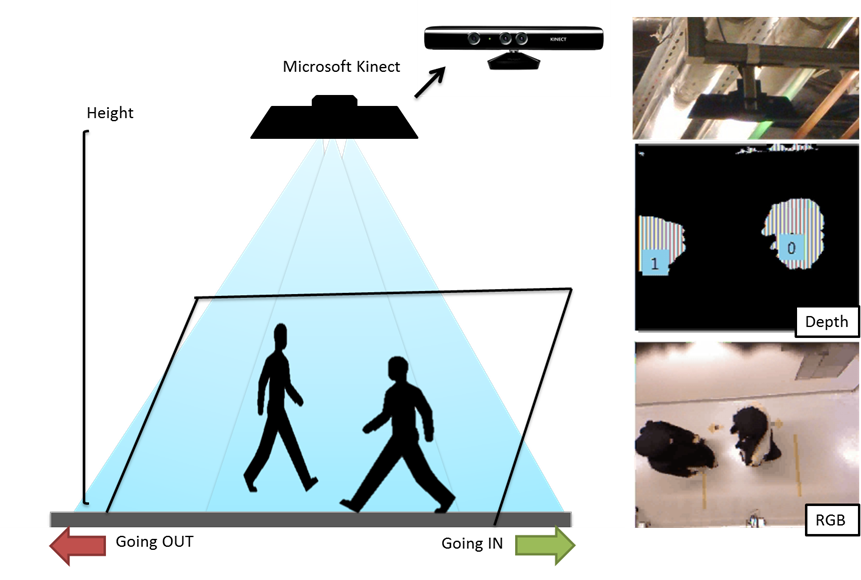
\includegraphics[width=1.05\columnwidth]{./images/minisys.png}
  \end{center}
  \caption{The architecture of our tracking system}\label{fig:minisys}
\end{figure}

People tracking through the Kinect sensor can be done using two methods:people tracking via human posture and an existing skeletal tracking by MSDN library. Both methods are implemented into our software to help us draw a fair comparison.

\begin{figure}[!ht]
  \centering
 	  	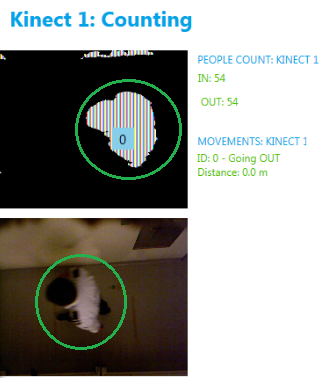
\includegraphics[width=0.7\columnwidth]{./images/darkview.png}
  \caption{Kinect sense even in dark view, which provide a high accuracy of data capturing}
\end{figure}

\subsection{Real World test-bed}
A human mobility detection system was implemented through a whole floor of a laboratory building. Since there might be difficulties and challenges in any deployment system, the sensors cover the most important parts/directions of lab areas that most students use. 7 Kinect sensors implemented in an I-smart laboratory at Masdar institute, the lab is occupied by 9 professors each supervising around 6-8 students.

\begin{figure} [!ht]
  \begin{center}
	  	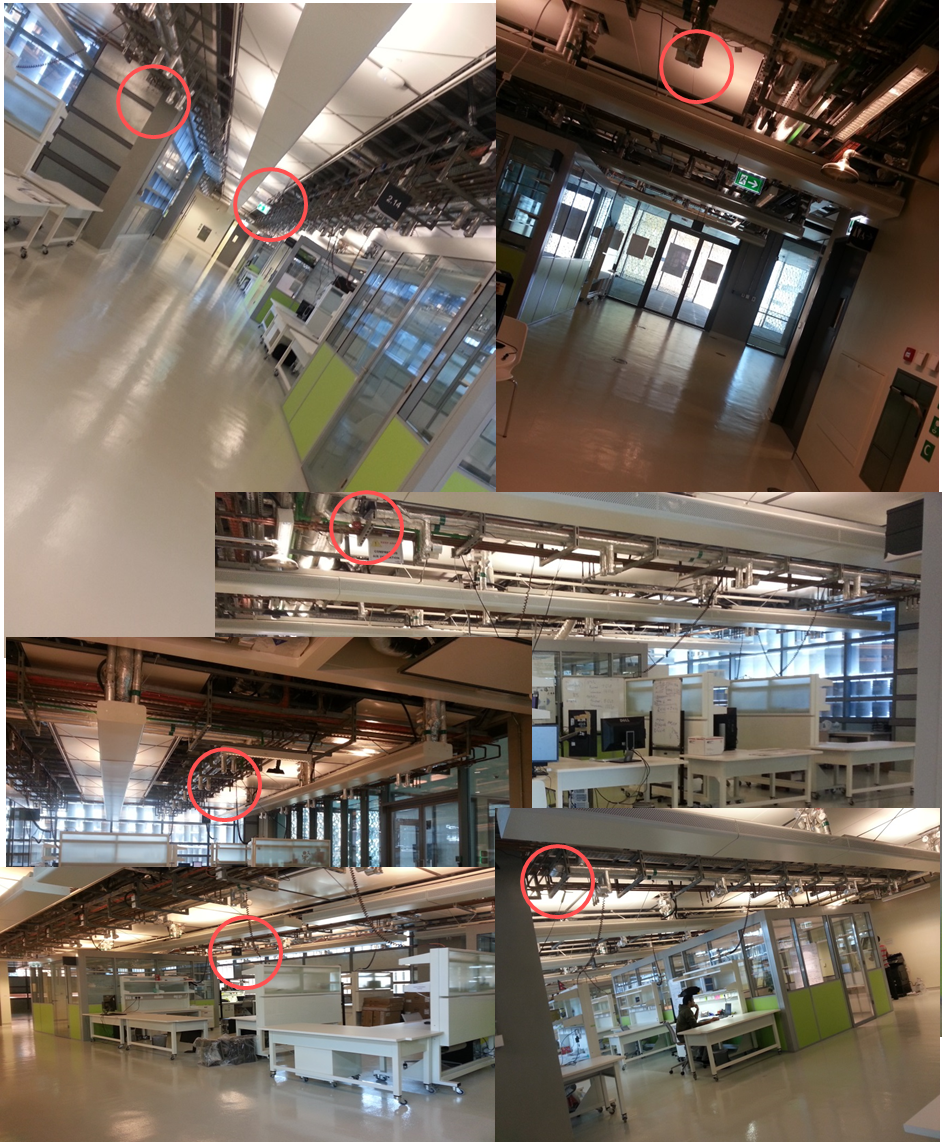
\includegraphics[width=0.9\columnwidth]{./images/realworld.png}
  \end{center}
  \caption{The real world test-bed }\label{fig:tstbd}
\end{figure} 

\subsection{The Markov Chain Model}
The prediction of the temporal dynamics of the occupancy in a zone is carried out using a Markov Chain (MC).  It represents the chain of states which a process goes through and is usually defined as a process which can be observed at a discrete set of times.  To design our observed data to easily fit the MC model, the number of occupants in each zone of the building is taken, and a threshold and a simple state is assigned to each observation after the threshold.

For example, let the number of zones be 3, and the occupancy in each zone be based on a threshold vector $(say [0, 5, 10, 15])$.  This assigns states like \\
${(E)mpty,  (F)ew,  (A)verage,  (C)rowd} $ to each zone.  i. e if in a zone the observed number of occupants (N) is zero then a state (E) is assigned to the zone.  Similarly, if $N > 0 $ and $N <= 5$, then the zone is assigned the state (F), for $N > 5 $ and $N <= 10$ ,  the state is (A) and so on.  For a sample observed occupancy data of the building with 3 zones occupancy data at time t, their corresponding state is $[8,.22, 0] \Leftrightarrow [F,  C,  E]$ .

Using the occupancy distribution at any time ${t}$ and the derived state vector, the state vector for time ${t + \triangle t}$  is predicted.  The predicted state vector for ${t + \triangle t} $,. allows  the prediction of zones that are likely to be more or less occupied.  A transition matrix is used to represent the probability of the transition from one state to another.  It is a two dimensional matrix encompassing the probability of all possible transitions  and refers to a square table with dimensions [Number of states X Number of states].   The element of the matrix at any location (i, j) is the probability of transition from $i^{th}$ state to $j^{th}$ state which is designated as $p _ {ij}$.   Figure \ref{fig:states} explains the state transitions drawn from equation \ref{equ:1} and the corresponding transition matrix of the three states representing the number of occupants in a building.

\begin{figure}[!ht]
  \centering
 	  	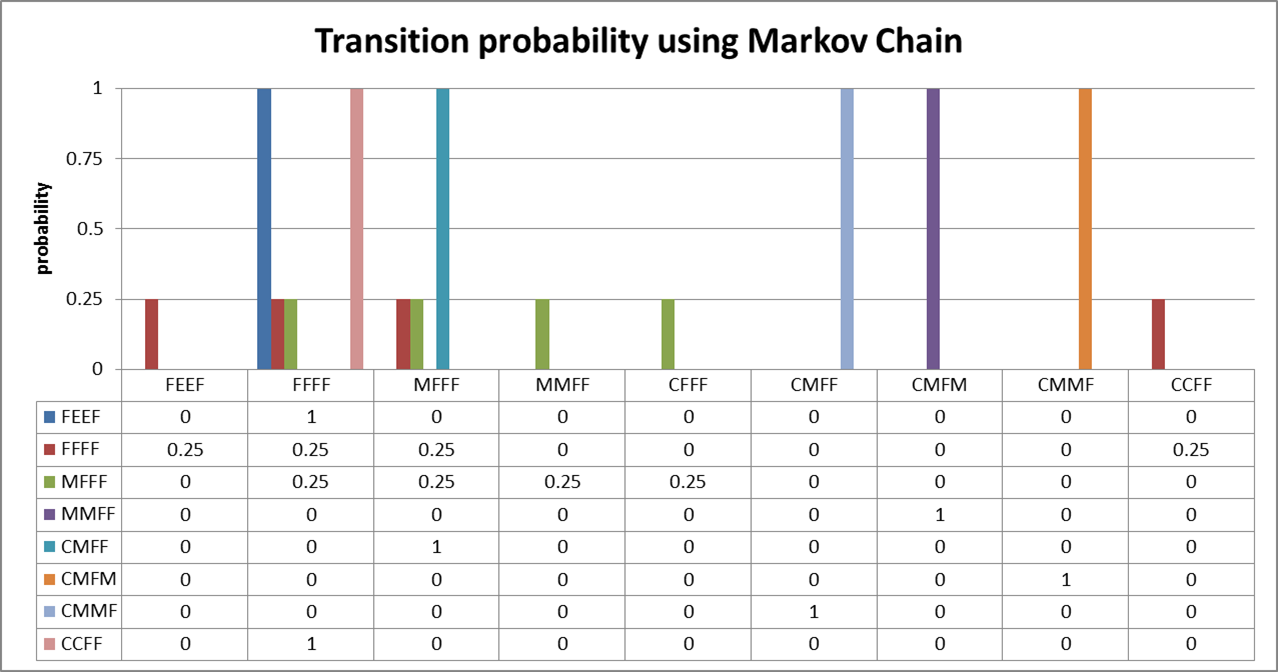
\includegraphics[width=0.9\columnwidth]{./images/mc.png}
  \caption{XXX}
\end{figure}

\begin{figure}[!ht]
  \centering
 	  	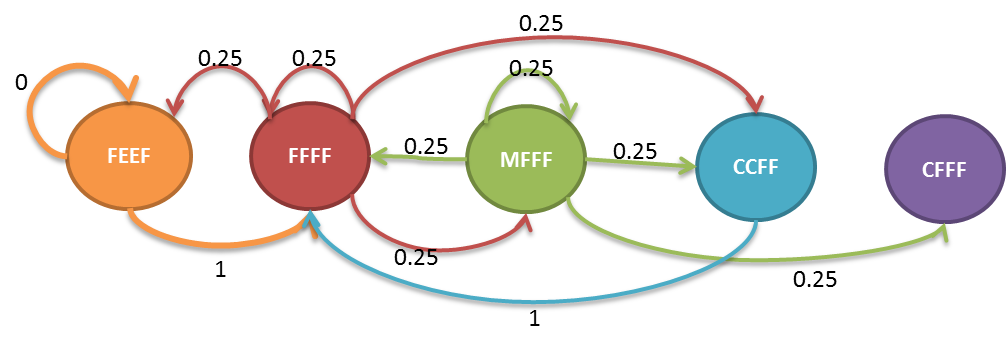
\includegraphics[width=0.9\columnwidth]{./images/mcc.png}
  \caption{XXX}
\end{figure}

\begin{figure}[!ht]
\centering
\resizebox{3.4in}{!}{%
\begin {tikzpicture}[-latex ,auto ,node distance =4 cm and 5cm ,on grid ,
semithick ,state/.style ={ circle ,top color =white , bottom color = processblue!20 ,
draw,processblue , text=blue , minimum width =1cm}]
\node[state] (C){$E$};
\node[state] (A) [above left=of C] {$F$};
\node[state] (B) [above right =of C] {$C$};
\path (A) edge [loop left] node[left] {$0.4$} (A);
\path (B) edge [loop right] node[left] {$0.1$} (B);
\path (C) edge [loop below] node[left] {$0.2$} (C);
\path (C) edge [bend left =25] node[below =0.15 cm] {$0.5$} (A);
\path (A) edge [bend right = -15] node[below =0.15 cm] {$0.3$} (C);
\path (A) edge [bend left =25] node[above] {$0.3$} (B);
\path (B) edge [bend left =15] node[below =0.15 cm] {$0.5$} (A);
\path (C) edge [bend left =15] node[below =0.15 cm] {$0.3$} (B);
\path (B) edge [bend right = -25] node[below =0.15 cm] {$0.4$} (C);
\end{tikzpicture}}
 \caption{ State diagram of Markov Chain with states Empty, Few or Crowded} \label{fig:states}
\end{figure}


\[
P=
  \begin{bmatrix}
  &Empty & Few & Crowded \\
Empty & 0.2&0.5&0.3\\
Few & 0.3&0.4&0.3\\
Crowded& 0.4&0.5&0.1\\
  \end{bmatrix}
\]


\begin{equation}
\begin{split}
\label{equ:1}
P( X _ {t+1} = s _ {t+1} | X _ t = s _ t ,  X _ {t-1} = s _ {t-1},
\ldots ,  X _ 0 = s _ 0 ) \\
= P( X _ {t+1} = s _ {t+1} | X _ t = s _ t )
\end{split}
\end{equation}

In P, all elements represent the probability of the transition from one state to another, including the same state.  For example, element $(2, 1)$ is the probability $P{21} = 0.4$ of the transition from the 2nd state which is (Few) to state 1 (Empty).  One of the main properties of the transition matrix is that the sum of all elements in any row equals 1.

\begin{equation}
\begin{split}
\label{equ:2}
\sum_{i=const, j=0}^{k-1} P_{i, j} = 1,   \\
 \text{Where k is the number of states}
\end{split}
\end{equation}

For any number of observations, the MC model can be easily applied to describe a single time step of event, i. e.  considering the present state (at t) the states at an immediate future time-step at ${t  + \triangle t}$  is described by the transition matrix.   In order to understand the probability of the transition from the present state to any particular state after n time-steps ${n \triangle t}$, then  we will use the following simple equation.

\begin{equation}
 \centering
\label{equ:4}
P_{ij}^{(n)} = \sum_{k=1}^{M} P_{ik} P_{kj}
\end{equation}

\subsubsection{Learning the Transition Matrix}
The entity that we are modelling is a dynamic process subject to changes with time. The transition matrix is built with occupancy data collected over time, in half an hour increment, in all registered zones.  For each zone, the probability of a particular transition (matrix element) is calculated by finding the ratio of the number of this transition with respect to the total number of transitions occurring.
\begin{equation}
 \centering
\begin{split}
\label{equ:5}
P_{ij} = n_{ij} \/ \sum_{k=1}^{M}  n_{ik} ,  \\
\text{Where m is the possible number of transitions}
\end{split}
\end{equation}


After building the transition matrix with a suitably large data set, it becomes possible to identify similar patterns in a new set of observations.

 Figure \ref{fig:occupflow} below shows the layout of a hypothetical office and the distribution of 7 Kinect sensors on its floors.
\begin{figure}[!ht]
  \centering
 	  	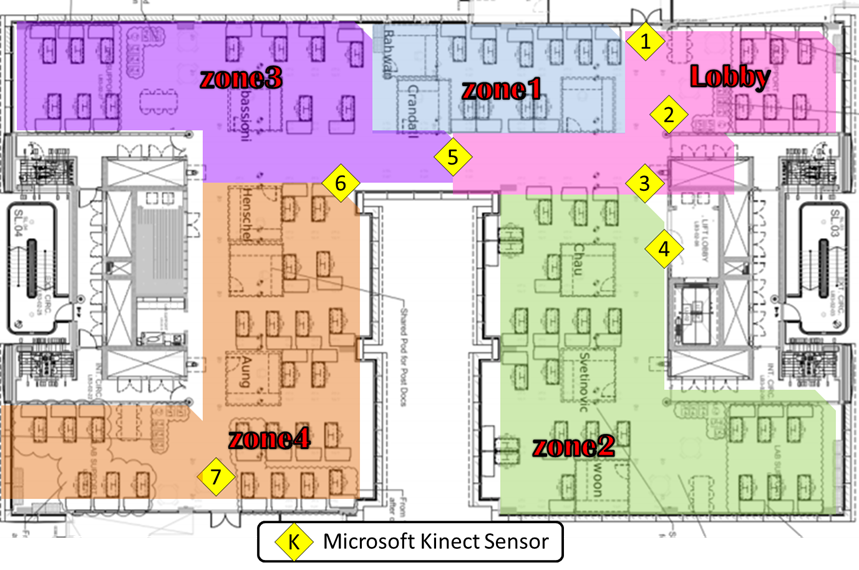
\includegraphics[width=0.9\columnwidth]{./images/numberofkinect.png}
  \caption{Distribution of 7 Kinect sensors on a building's floor layout.}\label{fig:occupflow}
\end{figure}

A log file is created in a format of the Table below \ref{table:logfile}:
 \begin{center}
\begin{table}[!ht]
  \centering
  \begin{tabular}{*6c}
08/10/2013& 22:51:30& IN:& 0 &OUT:& 1\\
08/10/2013& 22:51:31 &IN: &0 &OUT:& 2\\
08/10/2013 &23:30:30& IN: &0& OUT: &3\\
08/10/2013& 23:58:15 &IN:& 0 &OUT:& 4\\
09/10/2013 &05:17:21& IN: &1 &OUT:& 4\\
09/10/2013 &06:35:36 &IN:& 2& OUT:& 4\\
09/10/2013 &06:36:20& IN:& 2& OUT:& 5\\
09/10/2013 &07:09:11& IN: &3& OUT:& 5\\
09/10/2013 &07:15:04 &IN:& 3& OUT:& 6\\
09/10/2013 &07:25:46& IN:& 4& OUT: &6\\
\end{tabular}
\caption{Output log file for mobility tracking with exact timestamp at each sensor virtual gate.}
\label{table:logfile}
\end{table}
 \end{center}

This data is then parsed and converted into a different format in order to compute the effective occupancy of a zone.  The new format has 48 half hour time slots a day, and on each time slot the net people count is logged.

After counting the differences between the inflow and outflow of occupants, along with the previous estimate of the occupancy of each zone and the corresponding sensor gates, the net occupancy of each zone at a given time slot is calculated.

This data is related to the threshold vector [0, 5, 10, 15] and assigned one of the four states {E, F,  A, C}.   This data is referred to as the state matrix in \ref{table:stateslog}.
\begin{table}
  \centering

   \begin{tabular}{*5c}
Lab1&Lobby&Lab2&Lab3&Lab4\\
E&F&E&E&E\\
E&E&C&E&E\\
E&F&E&M&F\\
. &. &. &. &. \\
. &. &. &. &. \\
. &. &. &. &. \\
\end{tabular} \caption{Zone condition from occupancy data table.} \label{table:stateslog}
\end{table}

The number of possible states that can be observed in the building is equal to \ref{equ:6}
\begin{equation}
\label{equ:6}
\text{ ${(number of individual states)}^{(number of zones)}$}
\end{equation}

The total number of possible states of the building in this case is 1024,  from all 5 zones conditions of different element combinations of {E, F, A, C} ranging from {(E, E, E, E, E)}, {(E, E, E, E, F)}, {(E, E, E, E, M)} to {(C, C, C, C, C)}.

The transition matrix of size  [1024 X 1024], is then trained using the data above and the equation \ref{equ:5}, by counting the number of times a transition takes place divided by the total number of transitions.  There is a possibility that the input data set is not exhaustive in nature.  The transition matrix that is obtained is normalized row-wise to make the property in the equation true\ref{equ:2}.

After the matrix is trained, the implementation of the prediction system is simple and straightforward.  With new observations as the state matrix is updated with time, for any new row obtained, the state vector is taken say ({E, E, E, E, F}) and a one-time step prediction is made by finding the row number in the transition matrix which represents the state vector (row 2) and the column number with the maximum probability value is taken.  The state vector corresponding to the column number is the next predicted state of the building.

\subsection{Sample Model}

To understand how the problem is solved in-depth,  a sample date is observed and used to train the transition matrix. Let us consider a building floor consisting of two zones.  As the sensors observe the occupancy of each zone, with people entering or exiting any zone data is logged.  After parsing these log files, it is possible to obtain the occupancy of each zone in 48 time slots a day.   Table \ref{table:eee} formed for 12 slots  shown below is an example.
\begin{table}[!ht]
  \centering
      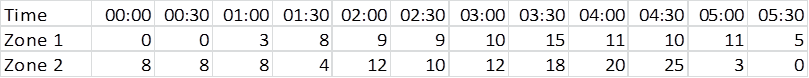
\includegraphics[width=0.9\columnwidth]{./images/t1.png}
  \caption{Example of occupancy data for two zones in a building.}\label{table:eee}
\end{table}

For thresholds, the occupancy matrix with a threshold vector [0, 5, 10] and assigning individual states {E, F, A, C} we get the table below \ref{table:vectort}:
\begin{table}[!ht]
  \centering
  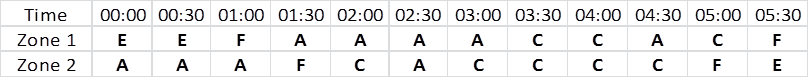
\includegraphics[width=0.9\columnwidth]{./images/t2.png}
  \caption{Representation of occupancy data, with transition condition.}\label{table:vectort}
\end{table}

For this problem, there are 16 possible combined states called state vectors.  The transition matrix that is formed is of size [16 x 16].  From the above table, we see that there are 11 transitions.  In a [16 x 16] matrix of zeroes,  for each transition observed the row number corresponding to the initial state vector is taken and the column number corresponding to next state vector is taken,  and the element at (row-number,  column-number) is incremented by 1.

Normalizing the transition matrix along the row, we get Table \ref{table:tmp} below:
\begin{table}[!ht]
  \centering
    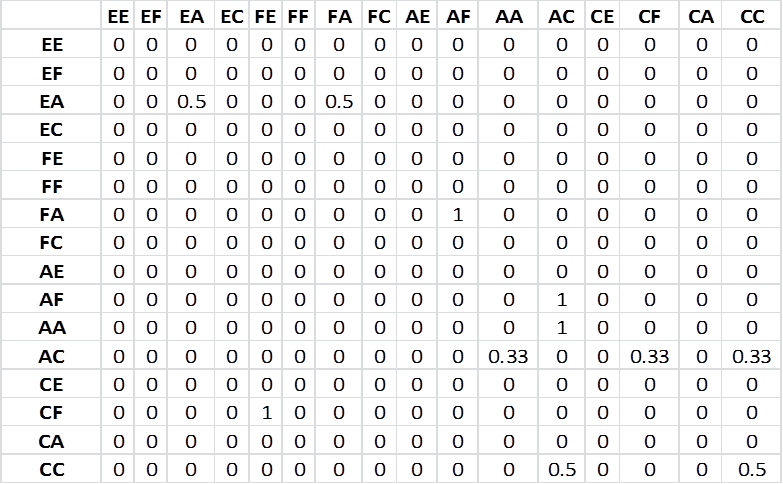
\includegraphics[width=0.9\columnwidth]{./images/t4.png}
  \caption{The transition probability between states.}\label{table:tmp}
\end{table}

The matrix has many empty rows, which shows that it is inadequately trained. After finding the transition matrix, the system is ready to predict future occupancy.  For an observation of [zone 1, zone 2] equal to say [8, 13], we get the state vector [A, C].  The next state of the building can then be obtained by taking the row MC and finding the index of the maximum element in the row, which is CA, with probability 0. 0929.



\section{Energy Consumption Analysis}
\label{sec:control}

\subsection{Occupancy Monitoring and Data analysis}

Occupants' mobility and behaviour in a building are important parameters in controlling energy consumption.  Occupancy data collected  must be analyzed first before serving as input to an energy controller. This data is initially collected by a Microsoft Kinect for Windows (K4W) sensor by our developed Occupancy-Counter software.


\subsection{Optimal control and planning}
The simplest control in an HVAC system is the cycling or OFF/ON control to meet partial load conditions. If the building only needs half of the energy that the system is designed to deliver, the system runs for some period, turns off for the next period, and then cycles on again. As the building load increases, the system runs longer and its off period is shorter. An alternative method of control under part-load conditions is staging. When conditions call for half the design capacity, only two units operate. At 60\% load, two units are base-loaded (run continuously), and a third unit swings (is either cycled or modulated) as needed. If it is assumed that Units 1 and 2 are base-loaded, and Unit 3 has just cycled on. The three ways of saving energy as mention in \cite{fnd} are then: Turn it OFF, Turn it DOWN or Turn it IN. The first refers to the first control method of cycling while the second refers to the staging usage, where part of the units are put on cycling and the other parts are operated with a low set-point. The last one refers to replacing or changing the air conditioning unit with a new one for more efficiency.

On the other hand, there are many other factors that play important roles in controlling air conditioning systems. These factors are:
\textbf{ The person thermal comfort:} There are different factors that influence thermal comfort including: clothing (level of cloths), activity level(human body release heats), air flow( direction of air), air temperature ( the level of cooling), and expectations( which vary from one person to another).
\textbf{ Space Size:} The small room size is different than a big one. The number of pieces of operating equipment is important since it releases some heat. To go on real-time controlling, it might consider the combined number of sensors that can include
\textbf{Space Design :}the number of windows and doors in the building. Windows bring the heat load from the sun and doors release the air out of the cooling space. More factors can be found in \cite{fnd}

\begin{figure}[!ht]
  \centering
 	  	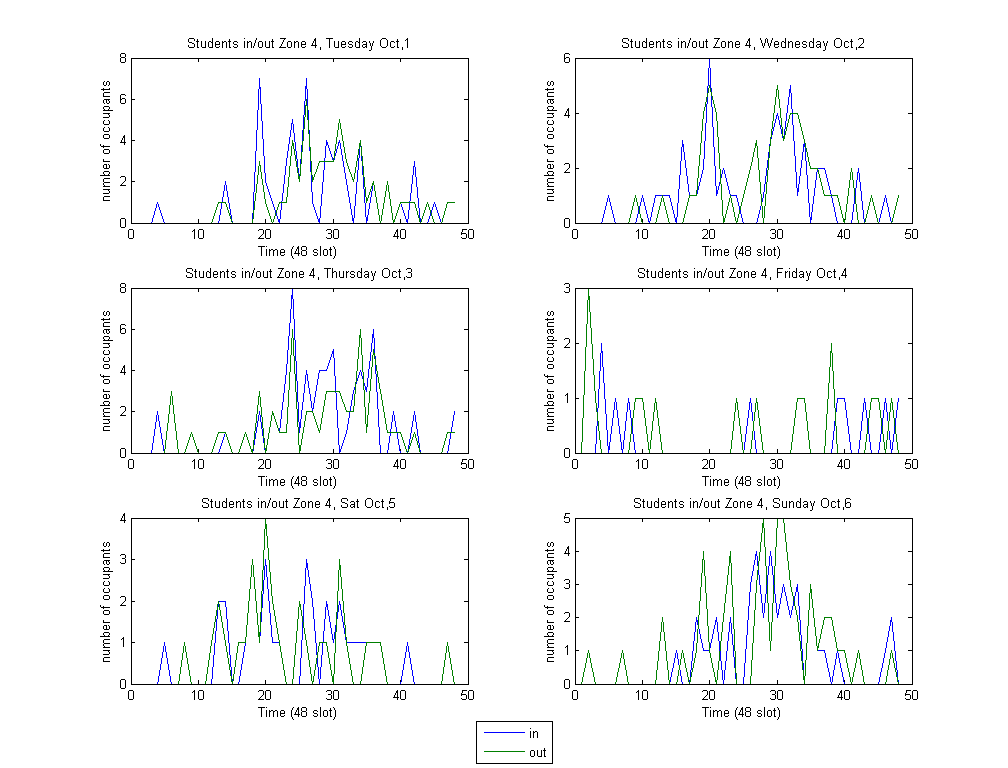
\includegraphics[width=0.9\columnwidth]{./images/occupancy.png}
  \caption{a week pattern of occupants mobility}
\end{figure}

\begin{figure}[!ht]
  \centering
 	  	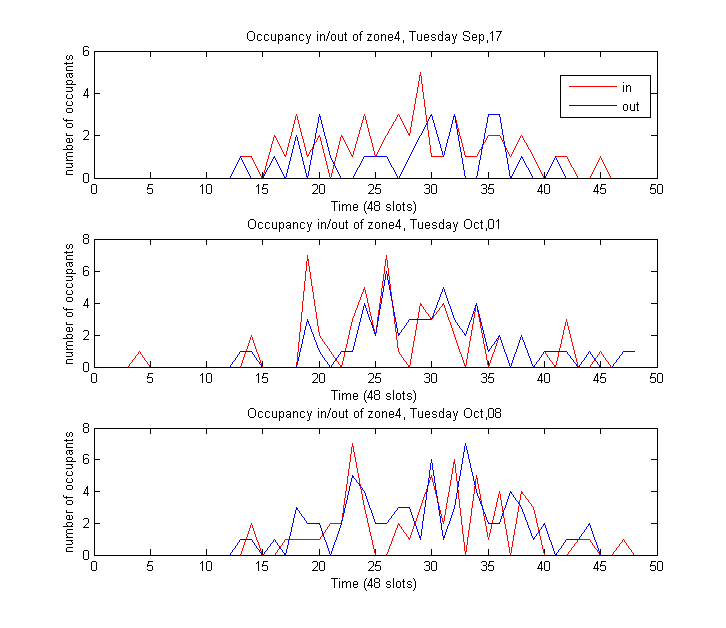
\includegraphics[width=0.9\columnwidth]{./images/tusday.png}
  \caption{a daily base pattern of occupants mobility}
\end{figure}

These automated control systems require full coverage of all above factors in order to say that air conditioning systems have been controlled efficiently. A system has been created that can display and show the occupancy time. A dynamic control method can be modelled from this system. As mentioned earlier, a Markov chain was used to create a matrix that predicted the future of moving from one state to another.  It is possible to benefit from these transition matrices by merging them to some controlling functions.It is possible to set the thermostat point to a certain point matching a certain event that occurs on the monitoring systems. Saying that, the probability to move from $state= (E,E,E,E)$ to $state=(E,A,E,E)$ after a hour will manage to open the air conditioning system at zone2 which represents the average occupancy one hour later. The remaining zones will maintain the temperature depending on the status information. This can be easily read from the display colours. The controller logic will work as a robotic command generator depending on the events created from our occupancy monitoring system. The main controller is programmable to keep a log for all states and zone conditions of the building. When some states occur they will generate new events which imply creating a control command to resolve the event issues.


\subsection{Simulation approach}
A net zero energy office building is simulated using the 'eQuest' building energy software adhering to Masdar Energy Design Guidelines (MEDG)based on the American Society of Heating, Refrigerating and Air-Conditioning (ASHRAE) 90.1. The office building is a two story building with a total floor area of $232m^2$. Each floor is divided into four office space with a floor area of $40m^2$ each. Windows are placed on the north, east and west walls of the building with overhangs having a projection factor (overhang depth/window height) of $0.6$. Two doors are placed on the north and east sides of the building. Windows and doors are not specified on the south wall to minimize heat gain through radiation. The window to gross wall area is kept at 29\%. The cooling system specified is a packaged direct expansion unit which delivers cooling through ducting.
The office space is designed for a total occupancy of 60 persons with $4.6 m^2$ per person. The air requirements are specified according to ASHRAE standard 62.1. The office space is specified as 20cfm/person(Indoor air quality method 2011) each.

\begin{figure}[!ht]
  \centering
 	  	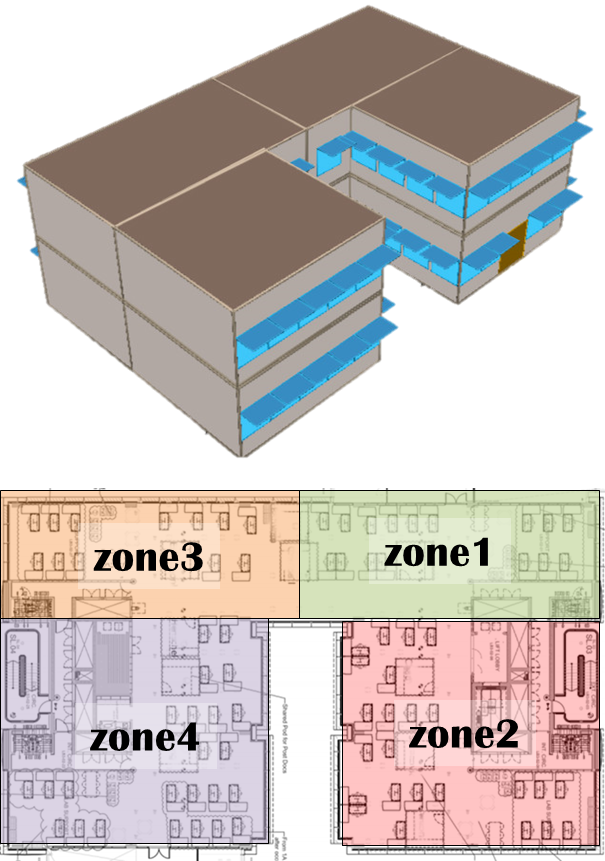
\includegraphics[width=0.9\columnwidth]{./images/zonedivided.png}
  \caption{The simulated Open Office looked like test-bed laboratory}\label{fig:simdesign}
\end{figure}


We demonstrate the potential energy savings for applying an occupancy schedule into controlling the HVAC running time. We used the Masdar Energy Design Guidelines (MEDG)\footnote{Masdar Energy Design Guideline (MEDG) as a baseline for occupancy and thermostat set-points. MEG has been created to specifically serve as a mandatory framework for designing energy efficient buildings in Masdar City.}

In the {\em first control case}, we tried to modify occupancy schedules and see the impact on energy consumption for space cooling.  The occupant's schedule  has by default one segment for weekdays and another for weekend. We substituted this schedule by a daily schedule  fed by data from our monitoring system. The potential energy saving difference between the two types of  scheduled  vs. unscheduled occupancy displayed in Figure \ref{fig:engsav}.

\begin{figure}[!ht]
  \centering
 	  	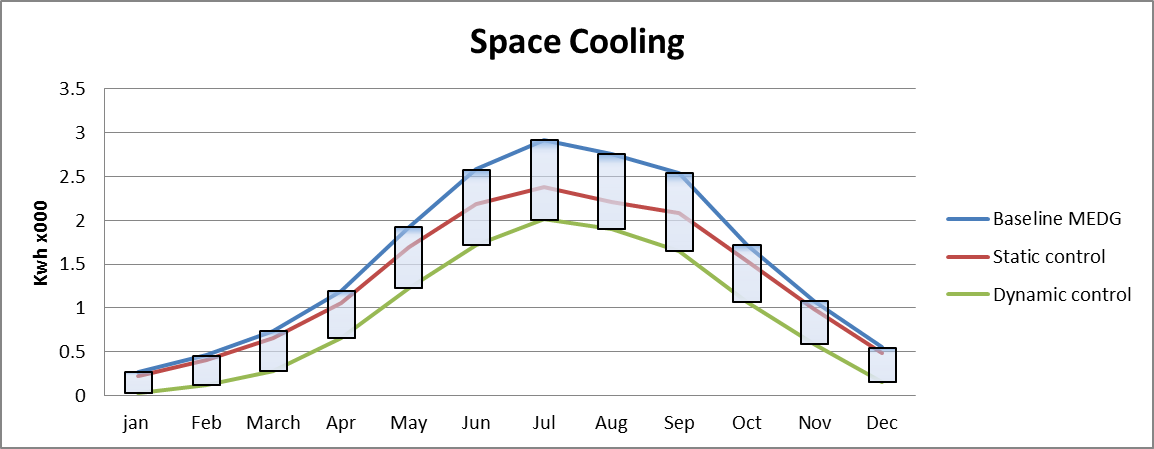
\includegraphics[width=0.9\columnwidth]{./images/sc.png}
  \caption{The simulated Open Office looked like test-bed laboratory}\label{fig:engsav}
\end{figure}

In the {\em second control case}, we modified the thermostat set-point schedule and convert it into more dynamic depend on our collected data. The set-point of thermostat is designed to meet the level of comfort, and here we rely on the occupancy density from our sample data to design customized set-point schedule for each day at different time. The results raise the energy consumption savings to 22.1\% as showing in figure  . There are a potential energy savings using customized occupancy/setpoint schedules. Even this small percentage of energy saving in favor of the custom schedule has a significant impact in large buildings. 


\subsection{Ventilation Rate}
Increase the number of occupants in a place may decrease indoor air quality. providing an appropriate thermal environment condition is important in maximizing worker productivity and minimizing discomfort level. As we notice in the baseline design, they assume a maximum number of occupants most of the time which increase the cost of ventilation rate Kwh. While, we could reduce this cost by applying a real occupancy schedule from real time occupancy monitoring system. The figure \ref{fig:vntrate} below shows a comparison between baseline vent. rate and Dynamic vent. rate depend on current occupancy sch.

\begin{figure}[!ht]
  \centering
 	  	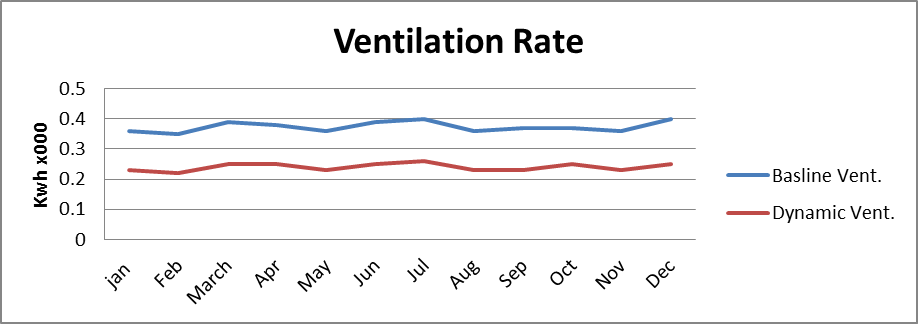
\includegraphics[width=0.9\columnwidth]{./images/vnt.png}
  \caption{Ventilation rate decreased by applying customized occupancy schedule}\label{fig:vntrate}
\end{figure}


\subsection{Temperature Outpoint}

\subsection{Thermal Conformability}

\begin{figure}[!ht]
  \centering
 	  	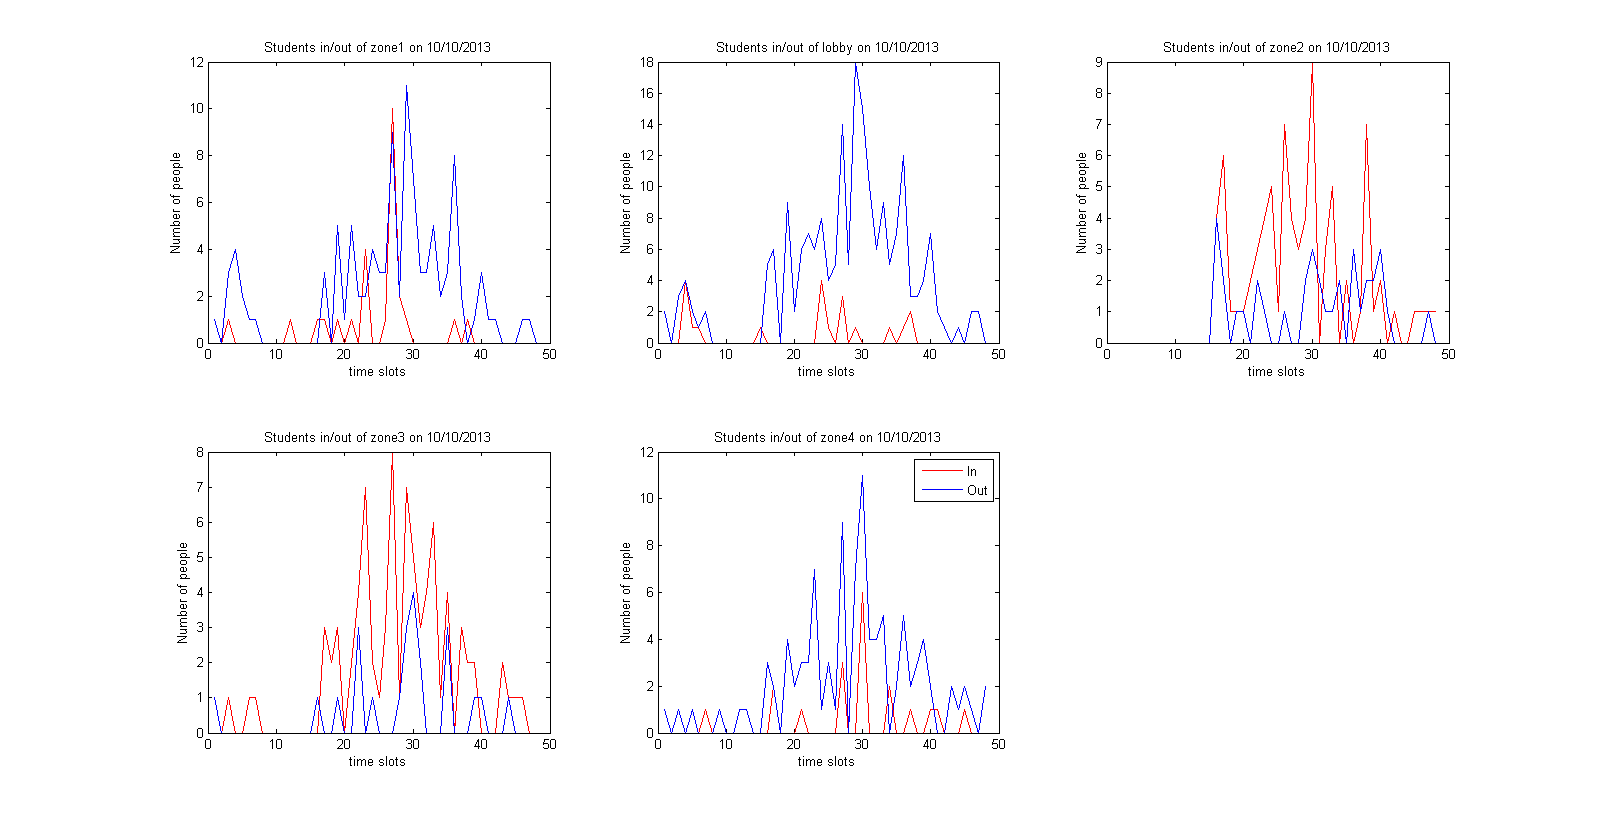
\includegraphics[width=1\columnwidth]{./images/inout.png}
\end{figure}

\begin{figure}[!ht]
  \centering
 	  	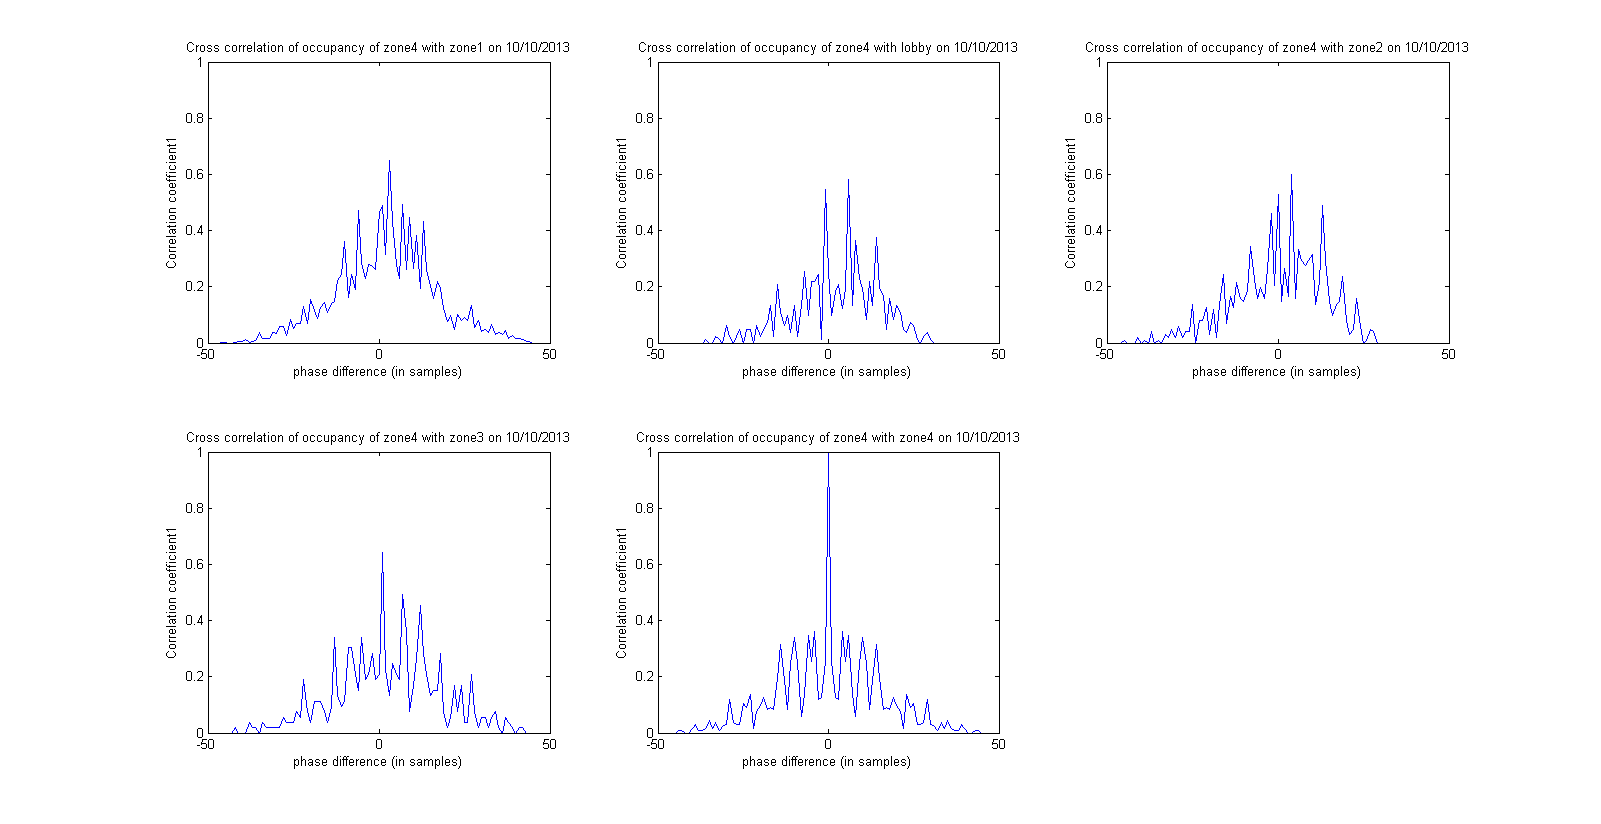
\includegraphics[width=1\columnwidth]{./images/crosscorrelation.png}
\end{figure}

\begin{figure}[!ht]
  \centering
 	  	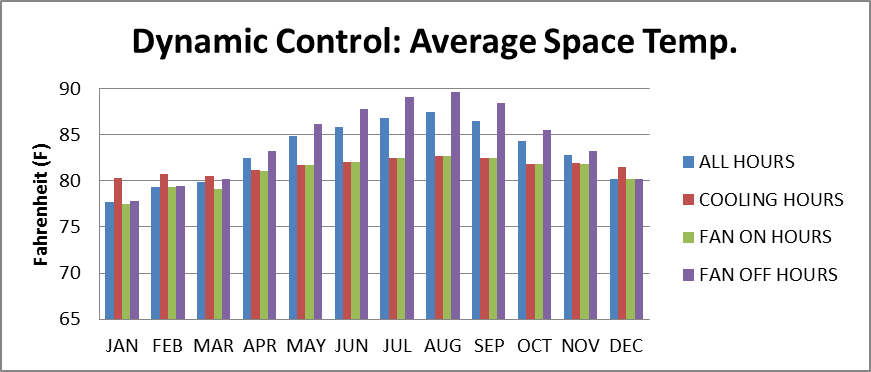
\includegraphics[width=1\columnwidth]{./images/temp.png}
\end{figure}

\begin{figure}[!ht]
  \centering
 	  	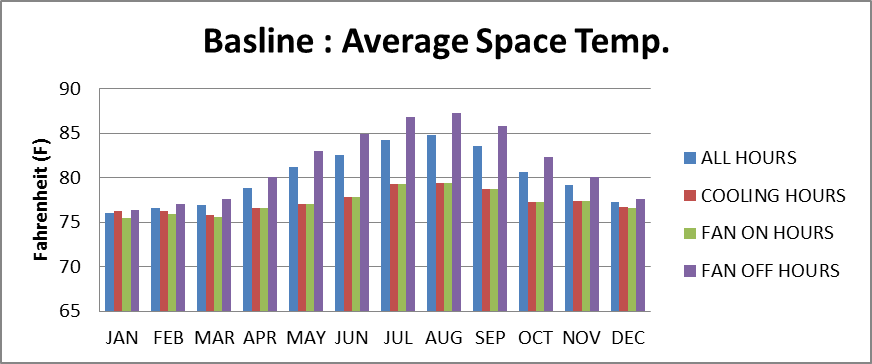
\includegraphics[width=1\columnwidth]{./images/temp2.png}
\end{figure}
\section{Related Works}
\label{sec:relatedworks}

The purpose of this section is to highlight works related to our approach in analysing human mobility. Building occupancy has been the subject of numerous studies for improving HVAC control. The following subsection gives more details.

\subsection{ HVAC control approaches}
There are a growing number of academic and industrial contributions to HVAC control strategies intended to reduce energy consumption in inhabited buildings. The majority of these contributions rely on occupancy models to produce occupancy simulations of an entire building. These simulations in turn would serve to calculate thermal loads with the intention of correctly provisioning the  HVAC system. There exist other remarkable approaches to HVAC control that start with the simple idea that occupancy can be inferred directly from the analysis of occupants’ movement within the different sections or outside of a building. There is neither requirement nor constraint on the number of occupants and zones. To this end, these approaches like in \cite{buildingoccupancyusingmarkov} implement a Markov chain method to simulate the occupant's movements. Here, the model is able to do two things with satisfaction: detect each occupant’s location and evaluate the occupancy rate in each zone of the building. In addition, it displays a realistic picture of daily building variation. Others put an emphasis on probability densities instead of making specific predictions. These models make no future projection about the likelihood of presence nor do they mention the actual number of occupants. For example, Page et al in \cite{stochasticsimulation}  model occupancy through a Markov chain. In this model, persons in particular zones of a building are modelled as time series simulating behaviour. In Page’s model, the main feature is the creation of an occupancy probability density on a daily basis.   The works of Liang and Lu deals with the aspects of combining human learning with power control strategies in the design of intelligent and malleable HVAC control strategies \cite{Designofintelligentcomfort}. Here, the authors used a minimum power control strategy which balances and reduces respectively the input power of an HVAC and the energy consumption. They also put into play six parameters : occupancy level, ambient and radiant temperatures, air strength, relative humidity, occupants’ clothing. Then, they designed a human learning strategy based on the Predicted Mean Vote (PMV) model. This allowed them to adjust the user’s comfort zone by learning his/her preferences. Fountain et al. were the first to introduce the idea of comfort zone in the design of control strategies in special occupancy contexts like hotels \cite{Comfortcontrol}. As explained above, comfort zone and human learning strategy have been applied together for thermal comfort control. In addition, Fountain used a Neural Network to circumvent the non-linear aspects of PMV calculation.   With a small number of rules in a Fuzzy System (FS), Arabinda has been able to create in \cite{invertedpendulum} a Neuro-fuzzy controller (NFC) which saves significant computational time. He first designed an FS containing 36 rules of which a few are used for training in a back propagation algorithm. Then, he applied neural network made of three layers of respectively 2, 30 and 1 neurons. This NFC exhibited a noticeable improvement in peak and time for transfer functions in the air supply models in ANF and PID controller. Alcal’a et al. acknowledge that FLCs (Fuzzy Logic Controllers ) are useful for the implementation of expert knowledge and control of HVAC systems. Here, it’s about using linguistic rules and facing the difficulty of the actual knowledge acquisition and elicitation when solving a particular HVAC control problem. They proceeded like with any expert system engineering. That is, a human expert in HVAC control was first extensively interviewed, his practical knowledge is extracted, elicited and then transformed into practical rules that make up an initial Knowledge Base (KB). Only a manageable number of control rules were necessary to partition the system because of the use of an expert knowledge.

The authors designed accurate models to simulate two experimental test buildings. Then the traditional controller was compared with the controller with genetically tuned parameters in the same context buildings during ten days. In the end, the controller studied was implemented and tested. As a result, not only was the level of thermal comfort the same as the traditional physical setting but there was a noticeable decrease in energy consumption by more than 10\%. In the same line of thought, Gacto et al. proposed in [21] an advanced evolutionary Multi-Objective Genetic Algorithm (MOGA) to increase the performance of HVAC system GA tuning of FLCs. Then, others have used an adaptation of MOGA to determine their effectiveness in fast convergence. Besides, an intelligent crossover operator and a GA technique for incest prevention (population diversity without unnecessary crossovers), have been used to improve the algorithm search ability. Using soft computing methods is a popular approach for automatic generation of rule-based fuzzy systems (Fuzzy RB).

\subsection{Building Occupancy Monitoring}
There are several occupancy-based methods that use multiple sources of sensory input. Some suggest that occupancy can be represented using linear regression models. Data gathered for lighting, material loads and occupancy is evaluated with a building walk through survey. A noticeable limitation of this model is its dependence on energy usage to detect the presence of a person. More often, its estimation of occupancy is weak specially when dealing with large groups in a conference room. The same remark is true about conditioning as with energy consumption. Sometimes, the EnergyPlus tool is used to estimate savings. Here a reactive strategy is used in adjusting temperature based on occupancy. In other occasions, door activity detection and PIR sensors for presence detection are used to distinguish the status of a home between occupied, unoccupied, occupants awake or asleep. The estimation of this model does not seem to consider ventilation which is a significant source of energy consumption and ignores daily schedules like an occupant’s activity on a Friday.

In the work titled Occupancy-Based Demand Response [30], the authors introduce an HVAC control strategy to achieve efficient conditioning. It relies on demand response and the real-time monitoring and occupancy prediction. In this occupancy based demand response approach, the authors describe an HVAC control strategy which utilizes a room occupant monitoring system. This system is able to detect in real time, the number of occupants of a room, infer its temperature and level of carbon dioxide (CO2). The most significant contribution of this research is the ability of this system to predict room occupancy. Prediction is necessary because it appears that in general, an HVAC system requires a little time to bring an ambient temperature to a certain level of human comfort according to the American Society of Heating, Refrigeration and Air-Conditioning Engineers. To achieve their goal, the authors  modelled room occupancy as a Markov chain by identifying each status of the room (level of occupancy, vacancy) as a state to which a transition probability is ascribed for moving to the next state (room status). From this model, occupancy includes ventilation and temperature control strategies which are then implemented in an EnergyPlus model. EnergyPlus is building energy simulation software with many innovative simulation features like heat balance-based zone simulation, distributed air flow, thermal comfort, water usage, outdoor ventilation, and solar systems. It is used to optimize design and save on heating, cooling, lighting, ventilation, other energy flows, and water use. For this purpose, it takes charge of parameters like the components of the HVAC system, the level of occupancy, the climate and the construction material.

\subsection{Model Predictive Control}
In contrast to many approaches that focus on general aspects described in the section above, there are a variety of predictive and adaptive models designed for medium size contexts like offices, labs and classrooms. In the contribution titled Network of Sensing, Learning and Prediction Agents  \cite{MamidiChangMaheswaran} the authors introduce a system of multiple adaptive sensor agents whose roles are to detect motion, read CO2, record sound level, ambient light and check door status (open, close). This innovative application called Building-Level Energy Management Systems (BLEMS) is in fact a multi-agent system made of fifty eight multi-modal sensors, scores of teach collaborative agents that adapt to occupants’ particular needs. In addition, it contains 74 actuators related to the building’s HVAC areas and two units for handling central air. In practice, patterns of occupants’ activity are acquired through observation. Then, HVAC operation is optimized in response to the occupant models. On the other hand, by creating an agent model of each occupant, it is possible to predict room occupancy rate. The purpose of this system is to create an appropriate balance between energy preservation and occupants’ comfort through the use of machine learning techniques in areas that are likely to be occupied. This system has been successfully deployed and able to estimate occupancy with a 95\% accuracy rate. The deployment setting is the premises of the University of Southern California (USC).

With OBSERVE, Erickson et al. show in \cite{EricksonCarreiraPerpinan} how to use a wireless sensor network to collect real time occupancy data and use it to create occupancy models. Such models may be included in a building system for control strategies. With occupancy model predictions drawn from a sensor network-based control strategy, the authors confirm that they have achieved 42\% annual energy saving without compromising the American Society of Heating, Refrigerating and Air-Conditioning (ASHRAE) comfort standards.  Xiang et al. present in the article Smart Personalized Office Thermal Control System (SPOT) \cite{SPOT} a smart personal thermal comfort system for use in an office environment. The role of this system called SPOT (Smart Personalized Office Thermal) is to find an acceptable balance between energy consumption and personal thermal comfort in an office environment. This is a reactive control strategy that takes into account real-time occupancy and personal thermal comfort. It rests on an original model of personal thermal comfort known as the Predicted Personal Vote (PPV) model. SPOT makes use of a collection of sensors including Microsoft Kinect to evaluate six parameters known to define human comfort: clothing, air speed, humidity, radiant temperature, and air temperature and activity level. These parameters are essential to the PPV model which guides SPOT in controlling heating and cooling parts that maintain comfort. In spite of its appealing features and effective results, the SPOT model of HVAC control has several inherent limitations related to the designers’ initial restricting assumptions like  spaces are thermally isolated from one another, confinement to a personal space, long lasting calibration process and the excessive cost of the systems.


\input{conclusion}





\bibliographystyle{plain}
\bibliography{bibliography}


\end{document}

